%==============================================================================
% DAHS -- IEEE conference manuscript (IEEEtran, conference mode).
% 6-page version. All figures are native LaTeX (pgfplots/TikZ); no external
% image files. Figure data traces to result files under results/ (the ground
% truth). Build:  pdflatex; bibtex; pdflatex; pdflatex
%==============================================================================
\documentclass[conference]{IEEEtran}

\usepackage{cite}
\usepackage{amsmath,amssymb,amsfonts}
\usepackage{amsthm}
\usepackage{textcomp}
\usepackage{booktabs}
\usepackage{pgfplots}
\pgfplotsset{compat=1.18}
\pgfplotsset{every axis/.append style={font=\footnotesize}}

\newtheorem{proposition}{Proposition}

\begin{document}

\title{Sample-Efficient Adaptive Heuristic Selection via Offline Rollout
Distillation for Dynamic Warehouse Order Dispatching}

\author{%
\IEEEauthorblockN{Vittal Mukunda}
\IEEEauthorblockA{Dept.\ of Industrial Engineering\\ and Management\\
R.\ V.\ College of Engineering\\
Bengaluru, India\\
vittalmukunda.im24@rvce.edu.in}
\and
\IEEEauthorblockN{Atharva Somani}
\IEEEauthorblockA{Dept.\ of Industrial Engineering\\ and Management\\
R.\ V.\ College of Engineering\\
Bengaluru, India\\
atharvasomani.im24@rvce.edu.in}
\and
\IEEEauthorblockN{Pranjal Malaiya}
\IEEEauthorblockA{Dept.\ of Industrial Engineering\\ and Management\\
R.\ V.\ College of Engineering\\
Bengaluru, India\\
pranjalmalaiya.im24@rvce.edu.in}
}

\maketitle

\begin{abstract}
\textbf{\textit{%
Dynamic order dispatching in deadline- and perishability-constrained warehouses
is routinely handled by simple priority rules, yet no single rule is best across
the operating conditions a shift passes through. A selection hyper-heuristic can
pick the right rule for the current context; the established ways of learning the
selector are, however, costly. Online reinforcement learning is sample-hungry and
unstable, and running a lookahead at every decision is too slow to deploy. We
propose DAHS, a selection hyper-heuristic trained by offline rollout distillation.
For each decision state in a corpus of simulated shifts we run short
truncated-horizon stochastic rollouts of every candidate rule and record the
per-rule cost vector; we then fit a calibrated gradient-boosted ranker to those
vectors. This amortises an expensive online lookahead into a one-shot, fully
offline supervised signal, and deploys as a single fast forward pass. We prove
that the truncated-rollout cost is a consistent estimator of the full-horizon
cost, with a truncation bias that decays in the rollout horizon, and confirm the
predicted bias-variance trade-off empirically. On 50 held-out simulated shifts,
DAHS attains a 1.33\% SLA-breach rate against 3.13\% for an analytic
one-step-lookahead controller and 3.73\% for an otherwise identical
snapshot-trained ranker, and is Pareto non-dominated across four load scenarios.
A faithful offline reinforcement-learning baseline reaches only 7.18\%, and DAHS
trained on one-tenth the data still outperforms it. DAHS trained on as few as 25
simulated shifts already outperforms both baselines at any training budget; we
position this sample efficiency as the central contribution.%
}}
\end{abstract}

\begin{IEEEkeywords}
Dynamic programming, dynamic scheduling, heuristic algorithms, reinforcement
learning, supervised learning.
\end{IEEEkeywords}

%==============================================================================
\section{Introduction}
\label{sec:intro}

Order dispatching on a warehouse floor is a sequential decision problem under
uncertainty: orders arrive stochastically, each carries a due date and possibly a
perishability constraint, and a small pool of pickers must be assigned work so as
to minimise late and spoiled orders. In practice the decision is delegated to a
\emph{dispatching rule}, such as first-in-first-out or earliest-deadline-first,
because rules are transparent, fast, and require no training. The well-known
difficulty is that no single rule dominates: the rule that minimises lateness
under light load is not the rule that does so when the queue is saturated or when
a burst of perishable orders arrives. A controller that \emph{selects} the rule
appropriate to the current state, a \emph{selection
hyper-heuristic}~\cite{drake2020hyperheuristics, dokeroglu2024hyperheuristics}, can
in principle capture the envelope of the pool without abandoning the operational
advantages of rules.

The open question is how to \emph{learn} the selector. The dominant modern answer
is deep reinforcement learning (DRL)~\cite{mahmoudinazlou2025drl}, which is
attractive but sample-hungry and unstable on problems where the per-state
advantage of one action over another is small relative to the return variance;
that is exactly the regime of rule selection. Imitation
learning~\cite{hanjung2025imitation} is a second answer. Both families face a
structural limitation: DRL never sees the counterfactual cost of the rules it did
\emph{not} take, and imitation needs an expert demonstrator. The training signal we
use has neither problem.

We take a different route. The cost of committing to a rule at a given state can
be measured directly by simulation: fix the state, run each candidate rule forward
for a short horizon, and record the cost it incurs. This is a
rollout~\cite{bertsekas2020rollout}. Rollouts are normally used online, re-run at
every decision, which is too slow for a warehouse controller. Our approach runs
rollouts offline, once, and uses them as a supervised training signal. For each
state in a corpus of simulated shifts we roll out every rule, obtain a per-rule
cost vector, and fit a supervised ranker to it. The expensive lookahead is thereby
\emph{distilled} into a cheap function approximator: at deployment the ranker is a
single forward pass, and the rollouts live entirely in the training set.

This paper makes three contributions. First, \emph{offline rollout distillation}
as a training paradigm: truncated-horizon stochastic rollouts of a fixed rule
pool, run once and offline, supply a per-state supervised target that avoids both
the per-decision cost of online rollout and the instability of online
reinforcement learning. Second, a \emph{consistency result}
(Proposition~\ref{prop:consistency}): the truncated-rollout cost is a consistent
estimator of the full-horizon cost, with a bias that decays in the rollout
horizon, which predicts, as confirmed empirically, that the horizon is the dominant
design choice. Third, a \emph{sample-efficiency result}: because the rollout
supplies a directly measured, low-variance per-state target, DAHS trained on 25
simulated shifts already outperforms a snapshot-trained ranker, an analytic
lookahead controller, and a faithful offline reinforcement-learning baseline
trained on ten times the data. We position sample efficiency, not the headline
breach margin, as the contribution of record. An ablation shows the soft
tempered-softmax label can be replaced by its hard arg-max with no measurable
change, so the working mechanism is the rollout and its horizon, not the
distributional objective.

%==============================================================================
\section{Related Work}
\label{sec:related}

\textit{Selection hyper-heuristics:} hyper-heuristics search the space of
heuristics rather than the space of solutions~\cite{drake2020hyperheuristics}; the
selection variant chooses, online, which low-level heuristic to apply, and is
surveyed in~\cite{dokeroglu2024hyperheuristics}. Dispatching-rule selection for
dynamic scheduling~\cite{durasevic2022dispatching} is the closest application
family. Prior selectors are typically trained by genetic programming, online
reinforcement, or hard-label imitation, whereas DAHS trains a supervised ranker on
rollout-derived per-rule cost vectors.

\textit{Rollout and approximate dynamic programming:} a rollout policy improves a
base policy by, at each state, simulating each candidate action followed by the
base policy and committing to the action of least simulated
cost~\cite{bertsekas2020rollout}. Rollouts are a cornerstone of approximate dynamic
programming~\cite{simchilevi2021adp} and are typically truncated to a finite horizon
for tractability~\cite{he2024truncatedrollout}. DAHS inverts the usual deployment:
rather than re-running rollouts online at every decision, it runs them once,
offline, to manufacture a supervised training set, encoding the per-rule cost vector
as a soft label via a tempered softmax, a label-distribution
representation~\cite{geng2016ldl}. Proposition~\ref{prop:consistency} is a
truncation-error argument in that tradition.

\textit{Learning-based dispatching:} deep reinforcement learning has been applied to
dynamic order picking~\cite{mahmoudinazlou2025drl}, order
batching~\cite{cheng2024drlhyperheuristic}, and warehouse
scheduling~\cite{zhang2024lstmppo}, and its scalability for production scheduling
remains under active investigation~\cite{stockermann2025drlscalability,
tassel2023rljssp}. We include a Proximal Policy Optimization~\cite{schulman2017ppo}
baseline at a matched budget and, separately, at a $60\times$ budget. Two recent
learning-based selectors are the closest competitors: imitation learning of
dispatching decisions~\cite{hanjung2025imitation}, which trains on the actions of a
single expert demonstrator, and offline reinforcement learning with maskable
action-value learning~\cite{pluijm2025offlineld}, which fits a value function from
logged data rather than regressing a directly measured cost.
Section~\ref{sec:results} compares against a faithful
fitted-Q~\cite{ernst2005fqi} instance of the latter, trained on the same logged
shifts. A recent review~\cite{sauer2025mlscheduling} frames bootstrapped
self-labelling as an emerging paradigm for machine learning in scheduling; DAHS is a
theoretically grounded instance of it.

\textit{Warehouse operations and simulation:} warehouse order-picking design and
control has a long literature~\cite{dekoster2007orderpicking, roodbergen2006layout,
boysen2019warehousing, boysen2025warehousing}. We evaluate in a discrete-interval
simulator; the simulation modelling and its verification and validation follow
standard methodology~\cite{law2000simulation, sargent2013vandv}. No prior work, to
our knowledge, combines truncated stochastic rollouts of a fixed rule pool as the
source of an offline supervised training set, a calibrated supervised ranker as the
deployed selector that sidesteps both the per-decision cost of online rollout and
the instability of online reinforcement learning, and application to deadline- and
perishability-constrained dynamic warehouse dispatching. DAHS occupies that
intersection.

%==============================================================================
\section{Problem Setting and Method}
\label{sec:method}

\subsection{The Dynamic Dispatching Problem}
\label{sec:problem}

We consider a single warehouse shift of length $T$ (8 hours). Orders arrive over
the shift; order $o$ has an arrival time $a_o$, a processing time $p_o$, an
absolute due time $d_o$, a perishability flag, and a priority class. A fixed set of
$m{=}10$ pickers processes orders, one at a time. Decisions are taken at the
boundaries of $N{=}32$ equal intervals of 15 minutes; at each boundary the
controller chooses a dispatching rule from a fixed pool, the chosen rule ranks the
queue, and pickers are assigned greedily down that ranking. The operator's
objective is a composite per-interval cost,
\begin{equation}
J = \frac{1}{N}\left( W_{\text{b}}\, n_{\text{b}}
   + W_{\text{t}} \sum_{o} \tau_o + W_{\text{u}}\, |Q| \right),
\label{eq:cost}
\end{equation}
where $n_{\text{b}}$ is the number of orders completed after their due time,
$\tau_o = \max(f_o - d_o, 0)$ the tardiness, and $|Q|$ the count of orders left
unprocessed at shift end. The weights $W_{\text{b}}{=}3.0$, $W_{\text{t}}{=}0.2$,
$W_{\text{u}}{=}0.005$ encode an operator who treats an outright SLA breach as the
dominant cost; they are fixed before any learning and not tuned to the method. The
environment is a deterministic discrete-interval simulator in which all stochastic
quantities are pre-sampled from a single seeded generator, making a shift
byte-identically reproducible from its seed, a property the rollout labeller
requires. Arrivals follow a homogeneous Poisson process at 1.65 orders/minute;
processing times and due-date offsets are triangular; a fixed 0.20 fraction of
orders are perishable. The pool holds four rules: FIFO (by arrival), FEFO
(first-expire-first-out), WSPT (weighted shortest processing time), and ATC
(apparent tardiness cost). As Fig.~\ref{fig:diversity} shows, all four win a
non-trivial share of decisions, so selection is a real problem.

\begin{figure}[t]
\centering
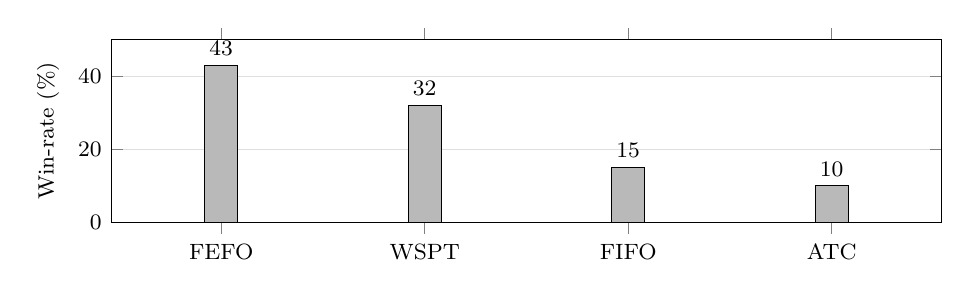
\begin{tikzpicture}
\begin{axis}[
  width=\columnwidth, height=3.9cm,
  ybar, bar width=12pt,
  ymin=0, ymax=50,
  ylabel={Win-rate (\%)},
  symbolic x coords={FEFO,WSPT,FIFO,ATC},
  xtick=data,
  nodes near coords, nodes near coords style={font=\footnotesize},
  enlarge x limits=0.18,
  ymajorgrids, grid style={gray!25},
]
\addplot[fill=gray!55, draw=black] coordinates
  {(FEFO,43) (WSPT,32) (FIFO,15) (ATC,10)};
\end{axis}
\end{tikzpicture}
\caption{Per-shift win-rate of each dispatching rule, the fraction of decision
states at which it is the cost-minimising choice. No rule dominates.}
\label{fig:diversity}
\end{figure}

\subsection{Rollout-Informed Training Labels}
\label{sec:labels}

We simulate 250 training shifts under a round-robin behaviour policy, yielding
$250 \times 32 = 8000$ decision states. The 25-dimensional state at each boundary
summarises queue length and its lags, queue age, critical and perishable
fractions, labour utilisation, mean slack and dispersion, orders at near-term
deadline risk, recent arrival rate, breach-rate lags, and temporal indices. For
each state $s_t$ we form a label over the four rules by truncated rollout: replay
the shift to interval $t$, then for each rule $h$ commit to $h$ and apply the base
policy for $\tau$ intervals, recording the cumulative cost
$\hat{J}^{\tau}_h(s_t)$. The cost vector becomes a distribution by a tempered
softmax,
\begin{equation}
p^{\tau}_h(s_t) = \frac{\exp(-\hat{J}^{\tau}_h(s_t)/\beta)}
                       {\sum_{h'} \exp(-\hat{J}^{\tau}_{h'}(s_t)/\beta)},
\label{eq:softmax}
\end{equation}
with $\beta$ chosen once so the median label entropy falls in $[0.3,0.7]$
($\beta \approx 4.38$). When the perishable fraction is below 0.05 the FEFO mass is
zeroed and renormalised. The deployed horizon is $\tau = 4$;
Section~\ref{sec:results} studies the choice.

\subsection{A Consistency Result for Truncated Rollouts}
\label{sec:consistency}

\begin{proposition}[Truncated-rollout consistency]
\label{prop:consistency}
Let $\bar{C}$ bound the composite cost in any single interval; such a bound is
finite because queue capacity and picker count bound per-interval breach,
tardiness, and unfinished count. Fix a state $s_t$ with $H_t$ intervals remaining.
For rule $h$, let $J_h(s_t)$ be the full-horizon rollout cost and
$\hat{J}^{\tau}_h(s_t)$ the $\tau$-truncated cost, $\tau \le H_t$. Then
\[
0 \;\le\; J_h(s_t) - \hat{J}^{\tau}_h(s_t) \;\le\; (H_t - \tau)\,\bar{C}
  \;=:\; \Delta_\tau, \qquad \forall h,
\]
and the truncated tempered-softmax label converges to the full-horizon label with
$\mathrm{KL}(p^{\infty}(s_t)\,\|\,p^{\tau}(s_t)) \le 2\Delta_\tau/\beta$.
\end{proposition}

\begin{proof}[Proof sketch]
The composite cost is a sum of non-negative per-interval contributions, so
truncation removes a non-negative tail spanning $H_t-\tau$ intervals, each at most
$\bar{C}$. Writing the label as a softmax of energies $-J_h/\beta$, the truncated
energies differ by at most $\Delta_\tau/\beta$; the log-sum-exp normaliser is
1-Lipschitz in the supremum norm, so each log-probability shifts by at most
$2\Delta_\tau/\beta$, giving the KL bound.
\end{proof}

Part one bounds the cost vector itself, so the consistency transfers to any label
derived from it, including the hard arg-max. The proposition has two testable
consequences. The bias $\Delta_\tau$ decreases monotonically in $\tau$, so a ranker
fit to longer-horizon labels fits a more internally consistent signal; the
cross-validated soft cross-entropy indeed falls monotonically with $\tau$. The
bound governs only the bias, though: estimating $\hat{J}^{\tau}_h$ from finitely
many stochastic rollouts also incurs variance that grows with $\tau$. DAHS
therefore faces a bias-variance trade-off in $\tau$, with an interior optimum that
Section~\ref{sec:results} locates at $\tau = 3$.

\subsection{Ranker, Regimes, and Controller}
\label{sec:ranker}

A Gaussian mixture fit to the training states (six components by BIC; mean pairwise
adjusted Rand index 0.998 over ten refits) appends six regime-membership
posteriors, giving the ranker 31 inputs. The ranker is a gradient-boosted
decision-tree classifier~\cite{chen2016xgboost} with four-class soft output, fit by
inverse-entropy-weighted replication so the objective is the Kullback-Leibler
divergence to the soft label. Hyperparameters are selected by 5-fold
shift-grouped cross-validation (18 configurations; depth 4, 500 trees, learning
rate 0.03; soft cross-entropy 0.677 against a uniform baseline of $\log 4 =
1.386$). Tree ensembles are not calibrated out of the box, so the output is
post-processed with isotonic regression on a 20\% held-out shift split, improving
the expected calibration error from 0.063 to 0.028 and the Brier score from 0.130
to 0.107, clearing a pre-registered 0.05 acceptance threshold. A thin switching
controller
applies the FEFO mask, enforces a minimum dwell of $T_{\min}{=}2$ intervals to
bound rule thrashing, and overrides the dwell when the ranker is highly confident.
It is a stability guardrail, not a performance driver.

%==============================================================================
\section{Experimental Setup}
\label{sec:setup}

All methods are evaluated on the same 50 held-out shift seeds, disjoint from the
250 training shifts. Beyond the default operating point, three scenarios stress the
method: low load, balanced, and high-load-perishable; parameters are fixed before
evaluation. We compare DAHS against the four static rules; \emph{snapshot\_xgb}, an
ablation identical to DAHS but with the horizon collapsed to $\tau = 1$, which
isolates the value of the rollout horizon; \emph{greedy\_mpc}, an independent
analytic one-step-lookahead controller that simulates each rule for one interval
and picks the cheapest; \emph{LinUCB}, a contextual bandit;
\emph{PPO}~\cite{schulman2017ppo} at a matched 8k-step budget (\emph{ppo\_fair})
and a $60\times$ budget (\emph{ppo\_full}); and \emph{offline\_fqi}, a faithful
offline reinforcement-learning competitor, fitted Q-iteration~\cite{ernst2005fqi}
with FEFO action masking, trained on the same 250 logged shifts under the same
behaviour policy, reward, and gradient-boosted-tree model class as the DAHS ranker.
The comparison therefore isolates the training signal, a directly measured per-rule
cost vector versus a single bootstrapped value, from the function approximator. The
primary KPI is the SLA-breach rate; we also report mean tardiness and the composite
cost of \eqref{eq:cost}. Uncertainty uses 10{,}000-resample bootstrap 95\%
confidence intervals; paired comparisons use the Wilcoxon signed-rank test with
Benjamini-Hochberg control of the false discovery rate.

%==============================================================================
\section{Results}
\label{sec:results}

\subsection{Main Comparison}
\label{sec:main}

Table~\ref{tab:main} reports every method on the default scenario. DAHS attains a
1.33\% SLA-breach rate; the nearest competitors are greedy\_mpc at 3.13\% and the
snapshot ($\tau{=}1$) ranker at 3.73\%. DAHS thus improves on the snapshot ablation
by 2.40 percentage points: the multi-step rollout, absent from the snapshot, is
doing real work. DAHS also attains the lowest composite cost. The offline
reinforcement-learning baseline reaches 7.18\%, behind even the snapshot ablation.
DAHS is Pareto non-dominated; no baseline beats it on every metric simultaneously.
FIFO clears orders aggressively for higher throughput, at more than four times
DAHS's breach rate. Across scenarios (Table~\ref{tab:scenario}) the picture holds:
DAHS is rank one at balanced and default load. Under high-load-perishable
saturation greedy\_mpc edges DAHS on breach by 0.59 points, the one cell DAHS does
not lead the breach metric, though DAHS keeps the lower composite cost there;
offline\_fqi instead collapses to a 61.9\% breach rate, more than three times DAHS.

\begin{table}[t]
\centering
\caption{Default scenario, 50 test shifts. Lower is better except throughput and
utilisation. The ppo\_full row coincides with FEFO because the 500k-step policy
collapses to always-FEFO.}
\label{tab:main}
\begin{tabular}{lrrrr}
\toprule
Method & SLA breach & Tardiness & Cost & Util. \\
\midrule
\textbf{DAHS (ours)}        & \textbf{0.0133} & 0.525  & \textbf{3.09}  & 0.936 \\
greedy\_mpc                 & 0.0313 & 1.822  & 9.19  & 0.846 \\
snapshot\_xgb ($\tau{=}1$)  & 0.0373 & 1.589  & 8.77  & 0.851 \\
ppo\_fair (8k)              & 0.0385 & 0.257  & 3.92  & 0.970 \\
FIFO                        & 0.0660 & 0.618  & 7.57  & 0.983 \\
LinUCB                      & 0.0694 & 5.208  & 23.61 & 0.771 \\
offline\_fqi                & 0.0718 & 0.531  & 7.46  & 0.960 \\
WSPT                        & 0.0949 & 10.671 & 43.56 & 0.686 \\
FEFO / ppo\_full (500k)     & 0.1181 & 0.997  & 12.60 & 0.947 \\
ATC                         & 0.1572 & 1.238  & 16.37 & 0.940 \\
\bottomrule
\end{tabular}
\end{table}

\begin{table}[t]
\centering
\caption{SLA-breach rate by scenario (50 test shifts).}
\label{tab:scenario}
\begin{tabular}{lrrrr}
\toprule
Scenario & DAHS & greedy\_mpc & snapshot & offline\_fqi \\
\midrule
low load             & 0.0000          & 0.0000          & 0.0000 & 0.0000 \\
balanced             & \textbf{0.00039} & 0.00546        & 0.00576 & 0.00342 \\
default              & \textbf{0.0133} & 0.0313          & 0.0373 & 0.0718 \\
high-load-perish.    & 0.1943          & \textbf{0.1884} & 0.1949 & 0.6192 \\
\bottomrule
\end{tabular}
\end{table}

\subsection{Sample Efficiency (the Central Result)}
\label{sec:sample}

The 2.40-point breach margin is, on its own, a modest empirical win. The result we
ask the reader to weight is how little data DAHS needs to reach it. We retrain DAHS
from scratch on budgets of 25 to 250 shifts (five replications each below 250) and
evaluate on the same 50 test shifts. Fig.~\ref{fig:sample} plots the outcome. DAHS
trained on 25 shifts attains a 1.44\% breach rate, already far below the snapshot
ranker (3.73\%) and greedy\_mpc (3.13\%). The curve is essentially flat from 25 to
250 shifts, so roughly 90\% of the training corpus is redundant. This is the
operational signature of rollout distillation: every training state carries a
directly measured per-rule target rather than the noisy, shift-level return an RL
agent must learn from, so the supervised signal is dense and low-variance and the
ranker saturates its learnable structure within a few dozen shifts. The
offline\_fqi baseline, by contrast, improves with budget but stays far above DAHS
and is still descending at 250 shifts (11.55\% at 25, 7.18\% at 250) with a
cross-replication standard deviation of 4.5 points at 25 shifts against 0.3 for
DAHS. DAHS from 25 shifts beats offline\_fqi from the full 250 by 5.7 points: a
deployable selector from one-tenth the data.

\begin{figure}[t]
\centering
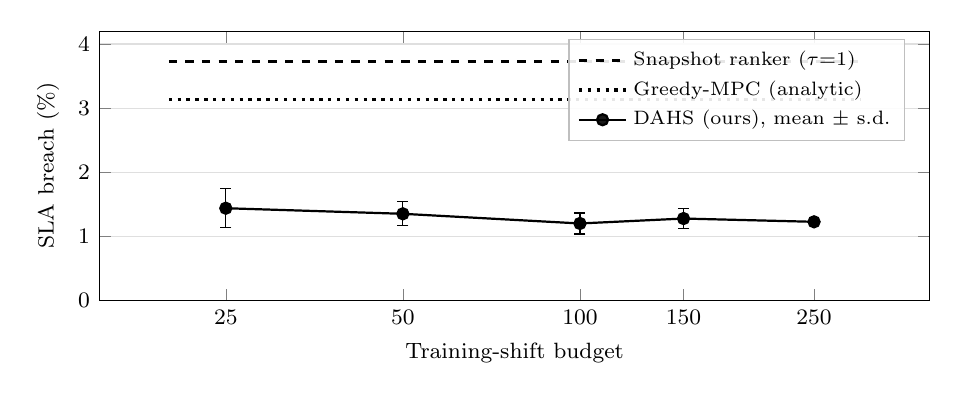
\begin{tikzpicture}
\begin{axis}[
  width=\columnwidth, height=5.0cm,
  xlabel={Training-shift budget}, ylabel={SLA breach (\%)},
  xmode=log, log basis x=10, xtick={25,50,100,150,250},
  xticklabels={25,50,100,150,250}, log ticks with fixed point,
  ymin=0, ymax=4.2, ymajorgrids, grid style={gray!25},
  legend style={font=\scriptsize, at={(0.97,0.97)}, anchor=north east,
                draw=gray!50, fill=white, fill opacity=0.9, text opacity=1},
  legend cell align=left,
]
\addplot[dashed, very thick, black, domain=20:300, samples=2] {3.73};
\addlegendentry{Snapshot ranker ($\tau{=}1$)}
\addplot[dotted, very thick, black, domain=20:300, samples=2] {3.13};
\addlegendentry{Greedy-MPC (analytic)}
\addplot[solid, thick, mark=*, mark size=2pt, black,
  error bars/.cd, y dir=both, y explicit]
  coordinates {
    (25,1.438) +- (0,0.302)
    (50,1.351) +- (0,0.189)
    (100,1.200) +- (0,0.164)
    (150,1.277) +- (0,0.156)
    (250,1.226) +- (0,0.000)
  };
\addlegendentry{DAHS (ours), mean $\pm$ s.d.}
\end{axis}
\end{tikzpicture}
\caption{Sample efficiency. DAHS SLA-breach rate versus the number of simulated
training shifts (mean $\pm$ standard deviation over five replications; zero at 250
because all replications draw the identical full corpus). DAHS trained on 25 shifts
already sits well below both reference baselines.}
\label{fig:sample}
\end{figure}

\subsection{Rollout Horizon, Robustness, and Ablations}
\label{sec:horizon}

Fig.~\ref{fig:tau} and Table~\ref{tab:tau} confirm the bias-variance trade-off of
Section~\ref{sec:consistency}. As $\tau$ rises from 1 to 4 the cross-validated soft
cross-entropy falls monotonically (0.817, 0.764, 0.709, 0.677), the bias term; the
operational breach rate, however, falls steeply to $\tau{=}3$ (1.05\%) and rises
slightly at $\tau{=}4$ (1.33\%), the variance term. The optimum is interior at
$\tau = 3$. Even the worst non-trivial horizon, the $\tau{=}1$ snapshot, is
$3.5\times$ worse than $\tau{=}3$: the rollout horizon is the single most important
design choice. Across a 12-cell robustness grid (four arrival rates crossed with
three deadline-tightness levels, only one calibrated) the method ranking is stable;
DAHS is no worse than the snapshot ranker in all 12 cells, no worse than greedy\_mpc
in 10 of 12, and no worse than offline\_fqi in all 12, by a margin that widens with
load. Degradation under heavier load is graceful and never collapses, whereas the
best static rule degrades to 70\% breach in the hardest cell.

\begin{figure}[t]
\centering
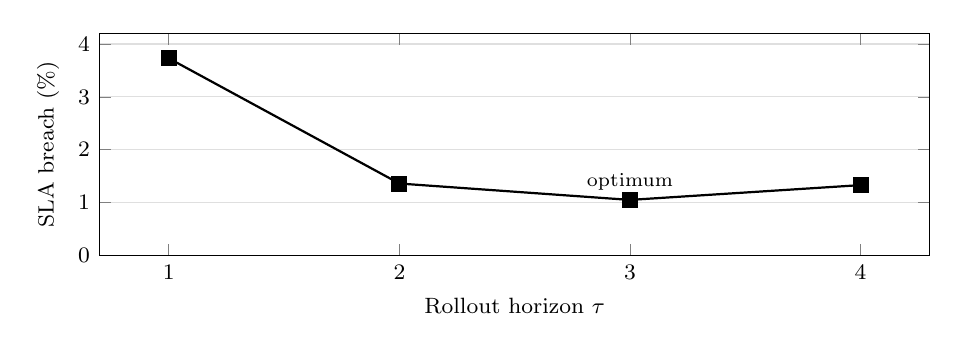
\begin{tikzpicture}
\begin{axis}[
  width=\columnwidth, height=4.4cm,
  xlabel={Rollout horizon $\tau$}, ylabel={SLA breach (\%)},
  xtick={1,2,3,4}, ymin=0, ymax=4.2,
  ymajorgrids, grid style={gray!25},
]
\addplot[solid, thick, mark=square*, mark size=2.5pt, black]
  coordinates {(1,3.73) (2,1.36) (3,1.05) (4,1.33)};
\node[anchor=south, font=\scriptsize] at (axis cs:3,1.05) {optimum};
\end{axis}
\end{tikzpicture}
\caption{SLA-breach rate versus rollout horizon. The U-shape, a steep improvement
to $\tau{=}3$ then a slight regression at $\tau{=}4$, is the bias-variance
trade-off of Proposition~\ref{prop:consistency}.}
\label{fig:tau}
\end{figure}

\begin{table}[t]
\centering
\caption{Rollout-horizon sensitivity (50 test shifts). The cross-validated soft
cross-entropy measures label fit; lower is better throughout.}
\label{tab:tau}
\begin{tabular}{lrrr}
\toprule
$\tau$ & CV soft cross-entropy & SLA breach & Composite cost \\
\midrule
1 (snapshot) & 0.817 & 0.0373 & 8.77 \\
2            & 0.764 & 0.0136 & 2.72 \\
3            & 0.709 & \textbf{0.0105} & \textbf{2.31} \\
4 (deployed) & 0.677 & 0.0133 & 3.09 \\
\bottomrule
\end{tabular}
\end{table}

Three ablations isolate single components. Replacing the soft tempered-softmax
label with its hard arg-max leaves the breach rate statistically unchanged (1.27\%
versus 1.33\%; $p = 0.11$) and the composite cost marginally lower, so the
distributional form of the label is not a source of DAHS's performance; the rollout
and its horizon are. Removing isotonic calibration degrades the breach rate to
2.94\% and the cost to 7.85 ($p < 0.001$), because the controller's entropy gate
acts on the predicted probabilities. Removing the switching controller slightly
\emph{improves} KPIs (breach 1.18\%, cost 2.74); we retain it deliberately, because
its role is to bound switching and enforce the perishability constraint, not to win
the comparison. A Shapley-value analysis~\cite{lundberg2017shap} attributes the
ranker's decisions to operationally sensible features: queue length and its lags,
mean slack, near-term deadline risk, and the interval index.

\subsection{Reinforcement-Learning Baselines and Real-Data Grounding}
\label{sec:rl}

Whether the deep-RL baseline is under-trained is a fair question; the evidence says
the issue is structural. At 8k steps PPO oscillates between two rules (3.85\%
breach); a $60\times$ budget makes matters worse, collapsing onto always-FEFO
(11.81\%). The per-state advantage of one rule over another is small relative to
the shift-return variance, so the policy drifts to the highest unconditional-return
rule. The offline baseline does not collapse at the default operating point: it
ties DAHS on tardiness (0.531 versus 0.525) and beats the snapshot and analytic
controllers on composite cost, yet loses the primary metric by 5.85 points
(95\% CI [3.85, 8.11]). An SLA breach is a rare, expensive event, and a scalar
bootstrapped value smears that signal across the bulk cost of tardiness and queue
volume; the per-rule rollout-cost vector measures the breach-laden cost directly.
We also validated the simulator's input distributions against the Olist Brazilian
e-commerce trace~\cite{olist2018dataset}: the due-date window matches well
(Kolmogorov-Smirnov $D{=}0.039$, normalised Wasserstein 0.036), while the real
inter-arrival stream is far burstier than Poisson ($D{=}0.153$, coefficient of
variation 2.68 versus 1.00, skewness 11.0 versus 2.0). Re-running
the full comparison with the frozen DAHS ranker under a bootstrap of the empirical
bursty arrivals, every method degrades, but DAHS retains rank one and its paired
margin over the snapshot ranker widens to 2.50 points (95\% CI [1.68, 3.45]). The
advantage is therefore not an artefact of the idealised arrival process.

%==============================================================================
\section{Discussion and Conclusion}
\label{sec:discussion}

The results support a narrow but well-grounded claim. On deadline-constrained
warehouse dispatching, a selector trained by offline rollout distillation is
sample-efficient, theoretically consistent in its training signal, and robust
across untuned operating points and a realistically bursty arrival stream. The
headline SLA-breach margin over the strongest learned baseline is real but modest;
we have been explicit that the contribution is the mechanism and its data
efficiency, not the size of that margin. DAHS helps most where rule selection is
genuinely contested: moderate-to-high load with tight deadlines, where the queue
state swings the best rule from interval to interval. It helps least at the
extremes, where every rule is adequate or the rules converge under saturation. Two
deployment properties reinforce the operational case. DAHS runs no simulation at
deployment, paying the lookahead cost once, offline, at labelling time, whereas the
analytic controller simulates every rule at every decision. And the action it emits
is one of four named rules a supervisor already understands, rather than an opaque
assignment; we scope this carefully, since the selector itself is a tree ensemble
interpreted only post hoc.

The broader methodological point is that an expensive online computation, the
rollout, can be paid once, offline, and amortised into a cheap learned
approximation, provided the offline computation becomes a supervised target rather
than a reinforcement signal. A controlled comparison supports the proviso: an
offline reinforcement-learning baseline given the same logged shifts, the same model
class, and a fair hyperparameter search, but trained to bootstrap a value, loses the
primary metric by 5.85 points. Limitations remain. Evaluation is simulation-only,
and pick time has no public real-world analogue; the simulator was calibrated at one
operating point, though the ranking is stable across eleven further untuned cells;
DAHS concedes the breach metric in the single saturation cell; and a modern
conservative offline-RL method (CQL, IQL) is left to future work, alongside
evaluation on a logged real-warehouse trace and an online variant that adapts the
rollout budget to the remaining horizon.

%==============================================================================
\bibliographystyle{IEEEtran}
\bibliography{references}

\end{document}
